 \documentclass[12pt,a4paper]{article}
\newcommand{\sepspace}{\vspace*{1em}}
\usepackage{graphicx}
\usepackage{newlfont}
\usepackage{xltxtra}
\usepackage{dcolumn}
\usepackage{apalike}
\usepackage{xltxtra}
\usepackage{marvosym}
\usepackage{mathrsfs}
\usepackage{amsmath,amssymb}
\usepackage{psfrag}
\usepackage{bm}
\usepackage{bbm}
\usepackage{latexsym}
\usepackage{fontspec}
\usepackage{multirow}
\usepackage{amssymb}
\usepackage{diagbox} %table split headers
\usepackage{longtable}
\usepackage{array}
\usepackage{rotating}
\usepackage{eqparbox}
\usepackage{makecell, caption, booktabs}
\usepackage{cellspace}
\usepackage{subcaption}
\usepackage{upgreek}
\usepackage[justification=centering]{caption}
\usepackage{lscape}
\usepackage[labelfont={bf}, labelsep=space]{caption}
\usepackage{float}
\floatstyle{plaintop}
\restylefloat{table}

\XeTeXlinebreaklocale "th"
\XeTeXlinebreakskip = 0pt plus 1pt 
\renewcommand*{\tablename}{Table}
\renewcommand{\refname}{}
\renewcommand{\baselinestretch}{2}
\renewcommand*\thesection{\arabic{section}.}
\renewcommand*\thesubsection{\hspace{0.5in}\arabic{section}.\arabic{subsection}}
\renewcommand{\refname}{\textsc{References}}
\bibliographystyle{apalike}


\setlength{\parindent}{0.5in}
\let\origdescription\description
\renewenvironment{description}{
\setlength{\leftmargini}{3.2em}
\origdescription
\setlength{\itemindent}{0em}}


% % % % % % % % % % % % % % % % % % % % % % % % % % % % % % % % % % % 

\begin{document}

\begin{figure}[t]
\vskip -1cm
\begin{center}

\includegraphics[width=3.5CM]{figure/SUT_Logo}
\end{center}
\label{fig:Logo}
\end{figure}
\begin{center}
\Large{Ph.D. Thesis Proposal}
\end{center}
\vspace{-0.1cm}
\begin{center}
{\textbf{\MakeUppercase{Silicon Sensor Design for Proton Computed Tomography}}}\\
\vspace{-0.1cm}
\LARGE{\textbf{\setmainfont{THSarabun.ttf}{การออกแบบเซนเซอร์ชนิดซิลิกอนสำหรับการสร้างภาพส่วนตัดด้วยอนุภาคโปรตอนโดยอาศัยคอมพิวเตอร์}}}
\end{center}
\vspace{0.5cm}
\begin{center}
BY
\end{center}
\begin{center}
\Large{Mr. Arnon Songmoolnak}
\end{center}
\vspace{0.5cm}
\begin{center}
SCHOOL OF PHYSICS
\end{center}
\begin{center}
INSTITUTE OF SCIENCE
\end{center}
\begin{center}
SURANAREE UNIVERSITY OF TECHNOLOGY
\end{center}
\begin{center}
March 2018
\end{center}

% % % % % % % % % % % % % % % % % % % % % % % % % % % % % % % % % % %
\thispagestyle{empty}
\newpage
\pagestyle{myheadings}
\begin{center}
\Large{Ph.D. Thesis Proposal}
\end{center}
\vspace{0.5cm}
\noindent Mr. Arnon Songmoolnak\hspace{4.35cm}ID. No. D5910212\\
\noindent \textbf{School of Physics}\hspace{5.3cm}\textbf{Institute of Science}\\
\noindent The Committee : \\
\indent A) Asst. Prof. Dr. Chinorat Kobdaj\hspace{2.1cm}Chairperson\\
\indent B) Dr. Todsaporn Fuangrod\hspace{3.5cm}Committee\\

\vspace{1cm}
\noindent\hspace{5.0cm}\begin{tabular}{l c}
Student's Signature & \hrulefill \\[-2ex]
 & (Mr. Arnon Songmoolnak) \\
 & 24 June 2019\\[1ex]
Advisor's Signature & \hrulefill \\[-2ex]
 & (Asst. Prof. Dr. Chinorat Kobdaj) \\
 & 24 June 2019\\%[1ex]
Co-advisor's Signature & \hrulefill \\[-2ex]
 & (Dr. Todsaporn Fuangrod) \\
 & 25 June 2019\\
\end{tabular}
\thispagestyle{empty}
\newpage
% % % % % % % % % % % % % % % section 1 % % % % % % % % % % % % % % %
\section{Thesis title}
\begin{description}
\item[\hspace{-0.3cm}]\MakeUppercase{Silicon Sensor Design for Proton Computed Tomography}
\item[\hspace{-0.31cm}] \Large{\setmainfont{THSarabun.ttf}{การออกแบบเซนเซอร์ชนิดซิลิกอนสำหรับการสร้างภาพส่วนตัดด้วยอนุภาคโปรตอนโดยอาศัยคอมพิวเตอร์}}
\end{description}

% % % % % % % % % % % % % % % section 2 % % % % % % % % % % % % % % %
% % % % % % % % % % % % % % % section 2 % % % % % % % %3 % % % % % % %
\section{Introduction}

Computed tomography (CT), is one of the most versatile diagnostic tools in clinical usages. It is also called ”computerized tomography” or ”computed axial tomography” (CAT).  The ability to create detailed images of internal organs such as bones, soft tissues, and blood vessels without any invasive surgery is the key advantage of this technology.  The fundamental principle of  CT is to use the x-ray to generate multiple cross-sectional images from a different angle and then reconstruct those multiple planes to three-dimensional images.  So the doctor, who uses the CT scan, can visualize three-dimensional organs and identify any potential problem occurs in such organs.  

Since the first x-rays were discovered in 1895 by Roentgen, it has been used for both medical and non-medical purposes.  Later in the 1920s, radiography and contemporary CT was included with x-ray.\cite{CTandXray}. 

X-ray radiotherapy and CT, which are referred to as conventional radiotherapy, exhibit some disadvantages when appl
ying to the hadron therapy (protons, neutrons and helium, carbon, oxygen and neon ions therapy) \cite{PToverRT} due to differences in their interaction properties with matters.  As an x-ray beam passes through the body, every tissue in the entire path will absorb energy from the beam. If the x-ray beam is used in clinical as the x-ray therapy to kill tumor cells, there are certain risks that tissues surrounding tumor cells can be exposed to unwanted x-ray energy. For example, the spinal cord or the optic nerve located near the tumor cell will get the unnecessary dose from the x-ray beam.

In contrary, proton therapy uses a positive charged particle or proton to treat tumor cells. This has an advantage over using the x-ray beam since it is possible to spare the surrounded tissues nearby tumor cells due to the Bragg peak figure \ref{fig:BraggPeak}.  In the existing proton treatment centers, x-ray computed tomography (CT) is still being used for locating tumor cells and performing dose calculations. But when it comes to the real treatment using the proton beam, the doctor and the medical physicist, who are responsible for the treatment planning, have to convert the formation obtained from the x-ray CT unit into the corresponding proton unit. This conversion, however, causes uncertainty in the tumor position due to systematic errors.  Using the proton beam for CT instead of x-ray can solve this systematic error issue and help doctors to connect with the proton treatment planning by enabling tumor position verification directly.\cite{PTinsteadrRT} 

 \begin{figure}[hbt]
\centering
  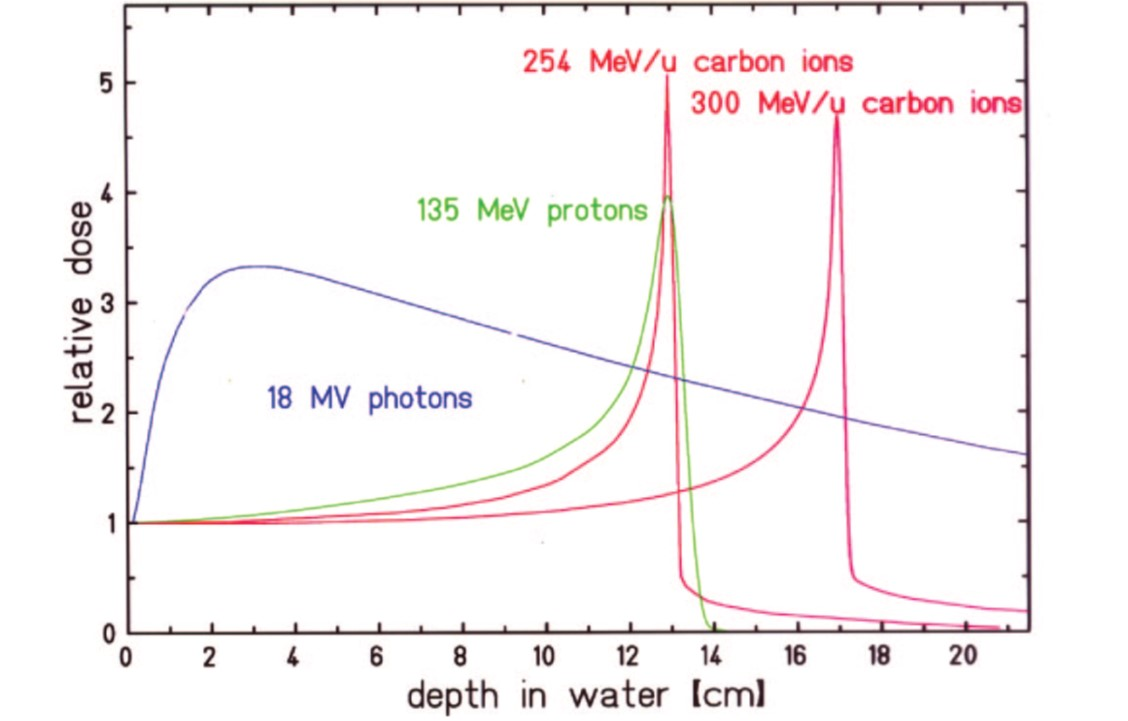
\includegraphics[width=10cm]{figure/BraggPeak.jpg}
  \caption{Depth-dose profiles of radiotherapy beams like photons, protons, and carbon ions\cite{BraggPeakImg}.}
  \label{fig:BraggPeak}
\end{figure}
 
Although, the first publication about proton radiography and computed tomography images were appeared in the late 1960s and 1970s,  the proton radiography (pRG) and tomography have been slow in development due to the   difficulties in generating the proton beam. It requires  a  sophisticated technology of either cyclotron or synchrotron.  In the 1960s, Cormack realized the possibilities of using the proton CT (pCT), and he proposed that the energy loss of protons passing through a patient can give important information about the proton stopping power that x-ray is unable to provide\cite{pRTandPCT}. 

Since then there were several attempts from various research groups to setup  prototypes for the pCT.  Most pCT systems being built consist  of four majors parts, position sensitive detector(PSD), residual energy range  detector (RERD), data acquisition with electronics readout unit  and image reconstruction software. 
An overview of a decade-long evolution of the conceptual design of pCT scanners and their calibration is given in the literature reviews section. For more details of   pCT scanner tests and performances for clinical applications in hadron therapy are presented  in\cite{BASHKIROV2016120}.

 \begin{figure}[hbt]
 \centering
  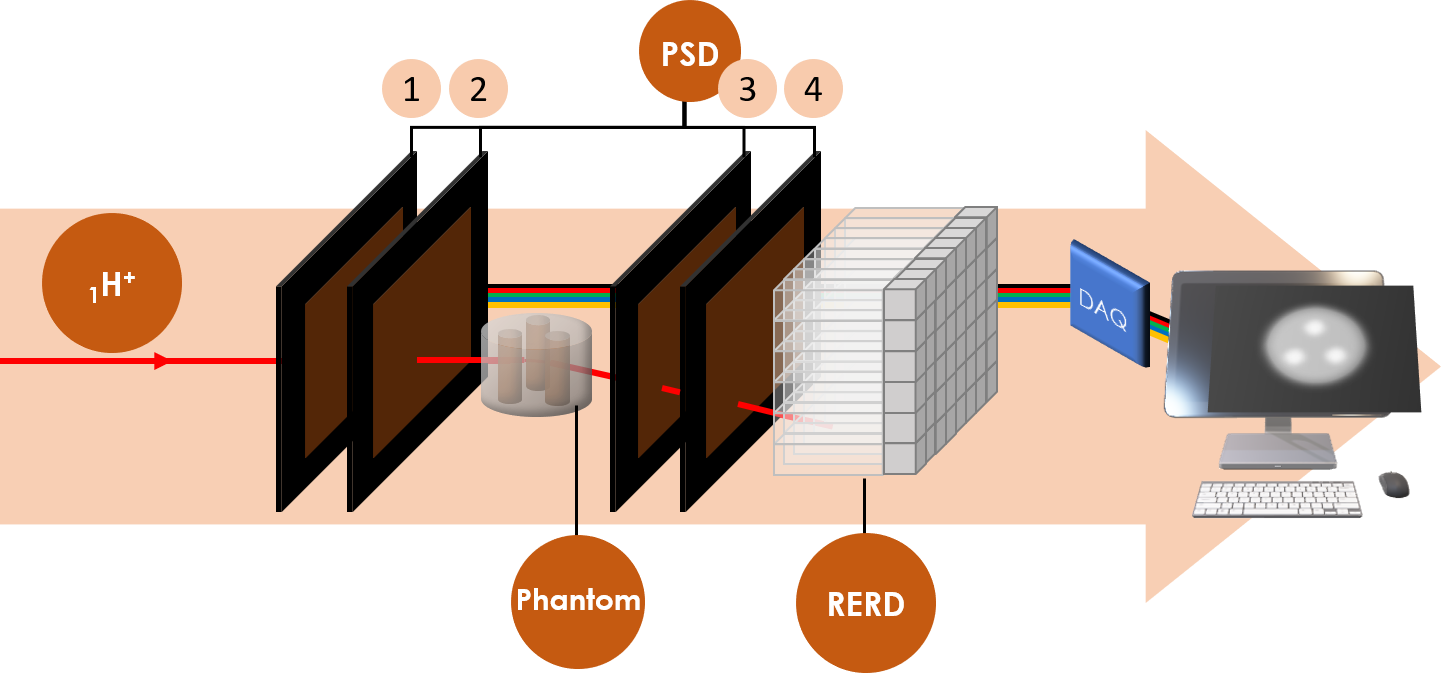
\includegraphics[width=10cm]{figure/PCT.png}
  \caption{The pCT scanner design concept based on individual proton tracking and energy measurement.}
  \label{fig:pCT}
\end{figure}

In the position sensitive detector (PSD), silicon pixel sensors are used for tracking the trajectory of a proton in the incident proton direction before and after entering a patient.  The sensors should have a large active area with a sub-mm pixel size, a fast frame rate, and a multiple-bit signal depth. Moreover, their read-out electronics should be able to resolve multiple protons in a single image frame.   To meet with above requirements,  the image sensors such as  the Complementary Metal Oxide Semiconductor (CMOS) \cite{CMOSinPCT} and the charge-coupled devices (CCDs) are being considered as suitable candidates. 

A conventional  Hybrid Pixel Sensor (HPS) is composed of a two-dimensional array of silicon sensor which is usually processed in high-resistivity of the silicon wafer and readout electronics with CMOS technology as shown in figure \ref{fig:HBS}. Each readout channel is connected with the active area which is the detecting element through a bump-bonding\cite{Broennimann:gf0003}.  While the charge-coupled device (CCD) is consisted of an insulating layer placed on the substrate along with the layer of insulation, electrodes, or taps. CCDs is design for transferring charge from one electrode to another.\cite{MATTIS1978355} 

Both HPS and CCD have high performances but their balance between granularity, material budget, radiation hardness, and read-out speed are not the best for high energy particle experiments.  In the propose of solving the disadvantage of CCD and HPS, the Monolithic Active Pixel Sensors (MAPS) shown in the figure \ref{fig:MAPS} is  introduced \cite{TURCHETTA2001677}. It integrates both electronics readout and sensor chip on the same piece of silicon wafer, provides better spatial resolution and being thin like CCDs.\cite{MAPS}

\begin{figure}[hbt]
    \centering
    \begin{subfigure}[b]{0.4\textwidth}
        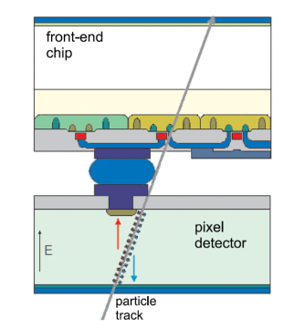
\includegraphics[width=\textwidth]{figure/HBS.png}
        \caption{Hybride Pixel Sensor.}
        \label{fig:HBS}
    \end{subfigure}
    \qquad
    ~ %add desired spacing between images, e. g. ~, \quad, \qquad, \hfill etc. 
      %(or a blank line to force the subfigure onto a new line)
    \begin{subfigure}[b]{0.5\textwidth}
        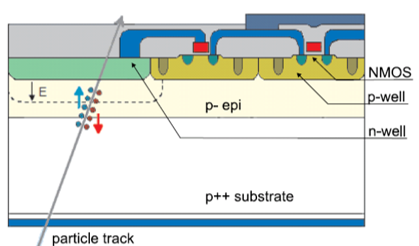
\includegraphics[width=\textwidth]{figure/MAPS.png}
        \caption{Monolithic Active Pixel Sensor.}
        \label{fig:MAPS}
    \end{subfigure}
    \caption{Pictures of Pixel sensors\cite{Suljic:2303618}}.\label{fig:ITS}
\end{figure}

Suranaree University of Technology (SUT),  Thai Microelectronics Center (TMEC) and Synchrotron Light Research Institute (SLRI) have been working together with A Large Ion Collider Experiment (ALICE), CERN,  in developing a  MAPS for the Inner Tracking System (ITS) upgrade project.  These MAPS will be mainly used for tracking particle trajectories after collisions.  The present version of ITS is called ITS1. It consists of six detector barrels with three different silicons technology, silicon pixel detector (SPD), silicon drift detector (SDD) and silicon strip detector(SPD). Now the second version or ITS2,  which is being constructed and will be installed in the year 2020,  consists only of silicon strip detector (SPD) called the ALICE Pixel Detector (ALPIDE).  Next for the third version or ITS3, it is in the beginning phase of research and development and schedules to be complete in the year 2026. The ITS3 is planned for a larger size of the sensor that can be bent into a shape of inner barrel as half cylinder\cite{ALICE-PUBLIC-2018-013}. 

Currently, ALICE is in the ITS2 commissioning period with ALPIDE chip being produced and installed on detector supporting structure.  ALPIDE  consists of active area and font-end circuity with the   28um x 28um  pixel size.   It is embedded with a 180 nm CMOS technology and fabricated on silicon wafer with a high resistivity of epitaxial layer. The area is 15 mm×30 mm and consists of 512×1024 pixels in matrix arrangement. Each pixel also composes of amplification, shaping, discrimination and multi-event buffering. The readout circuit reads the hit on sensitive area. The hits on pixel cause the signal within the pixel. The experiment requires more than 99\% of detection efficiency, the probability of fake-hit below 10$^5$ and 5 $\mu$m of a spatial resolution. The ALPIDE provides the read out for Pb–Pb interactions at 100 kHz. The power density of a chip is less than 35 mW/cm$^2$.\cite{SNOEYS2018}


\begin{figure}[hbt]
    \centering
    \begin{subfigure}[b]{0.3\textwidth}
        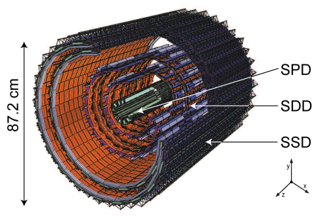
\includegraphics[width=\textwidth]{figure/ITS1.png}
        \caption{\centering ITS1 at 2013/2014 \cite{Aamodt:2010aa}}.
        \label{fig:ITS1}
    \end{subfigure}
    \begin{subfigure}[b]{0.3\textwidth}
        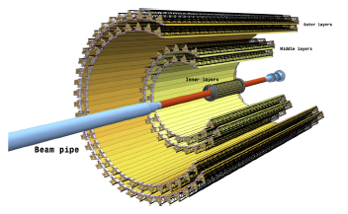
\includegraphics[width=\textwidth]{figure/ITS2.png}
        \caption{\centering ITS2 at 2018/2019 \cite{MAGER2016434}}.
        \label{fig:ITS2}
    \end{subfigure}
    \begin{subfigure}[b]{0.3\textwidth}
        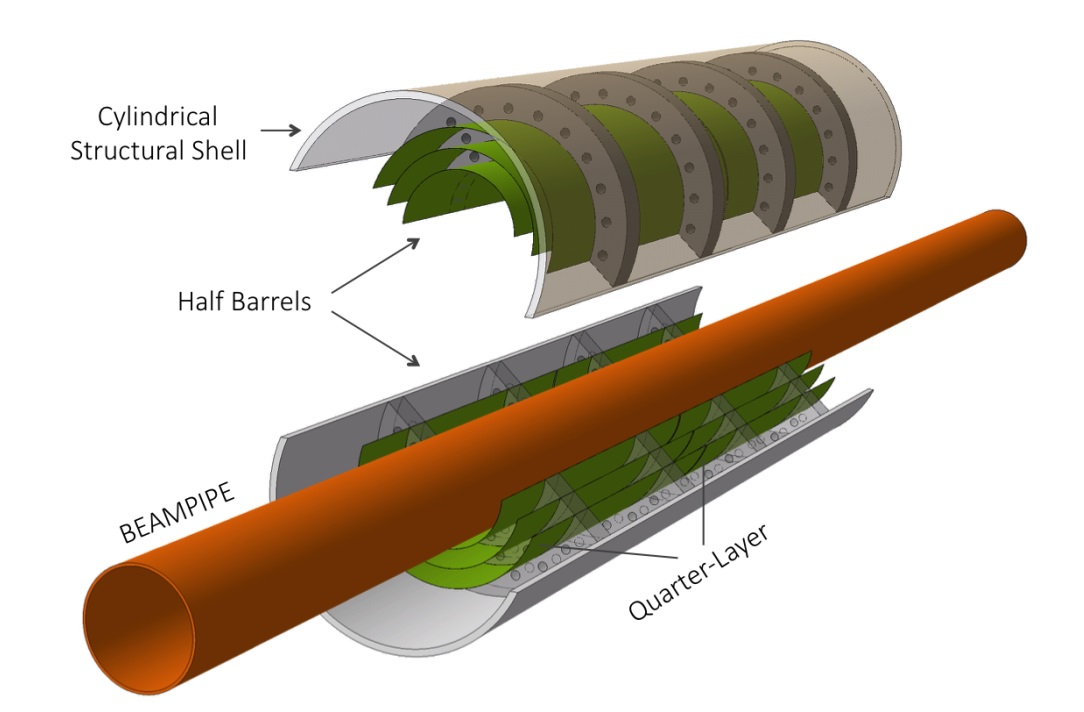
\includegraphics[width=\textwidth]{figure/ITS3.jpg}
        \caption{\centering ITS3 at 2025/2026 \\(ALICE, 2018)}.
        \label{fig:ITS3}
    \end{subfigure}
    \caption{Pictures of ITS}\label{fig:ITS}.
\end{figure}

To characterize the properties of the ALPIDE, SUT and SLRI have set up and developed the particle Telescope at SLRI Beam Test Facility (BTF). At the BTF, the measurements of hit positions, cluster size and detection efficiency of the ALPIDE pixel sensor chip have been performed\cite{SLRIandALPIDE}. The functionality tests(Laboratory tests) for electronics responses of each chip are also verified before installed into the particle telescope at the BTF. At present, there are several groups of researchers, who have been working with the ALPIDE chip including SUT, have proposed to use the ALPIDE in the PSD for the pCT prototype.  

In this proposal, we would like to study limitations of  the ALPIDE currently being used for the PSD part in the pCT prototype proposed by collaborating with a group at University of Bergen. Then, we will use these information as inputs for  designing a new silicon sensor based on MAPS technology together with teams from TMEC and ALICE for a prototype of the new pCT scanner. 

% % % % % % % % % % % % % % % section 3 % % % % % % % % % % % % % % %

\section{Research objectives}

The goal of the sensor design for the proton computed tomography project is to design the new prototype of pCT sensor for position sensitive detector (PSD) by observing the limitation of ALPIDE sensor in the prototype similar to the one proposed by University of Bergen and testing with the proton beam at King ChulalongKorn Memorial Hospital (KCMH).   Beside, we will design the new MAPS sensor by accommodating the requirements suggested by the innovative Medical Protons Achromatic Calorimeter (iMPACT) \cite{MATTIAZZO2017664} , which are 
\begin{itemize}
\item The pCT sensor should be able to detect at least  $10^9$ protons per a second with the read out rate more than 10 MHz/cm$^{2}$.  
\item The thickness of the sensor is expected to be lower than 50 $\upmu m$ to reduce the coulomb multiple scattering effect.
\item The sensor detection area should be greater than 16 cm$^2$ to cover the size of the patient body. If the sensor is small, one has to make an array of sensors to obtain the full coverage. This causes  the dead edge area around the connection between sensors.
\item The power consumption should be less  than 50 mW/cm$^2$ in order to avoid using of the cooling system. This would make the pCT system compact  and easily be integrated into the proton therapy system and possible to be able to use in the real clinical environment.
\end{itemize}
The design of  a new sensor will use above requirements as a starting point. The model and device simulation will be done by  using Sentaurus TCAD  Synopsys  at TMEC.   
% % % % % % % % % % % % % % % section 4 % % % % % % % % % % % % % % %
\section{Literature Reviews}

There are several  organizations and research institutes have designed and  constructed pRad and pCT therapy facilities with their own designs and concepts as shown in the table \ref{table:prototype}. Currently, there are four main  tracking technologies being implemented  Scintillator Fiber Hodoscope (Sci Fi) at Paul Scherrer Institute (PSI), Gas Electron Multiplier (GEM) at  Advanced Quality Assurance (AQUA), Silicon Strip from  the PRIMA collaboration, and Pixel Sensor (ALPIDE) in the innovative Medical Protons Achromatic Calorimeter \& Tracker (iMPACT)

\begin{table}[ht]
%\caption{ The table shows the organization collaborations}
\captionsetup{justification=justified}
\caption{ The table shows the organization collaborations to develop pCT and pRad prototype with proton tracking technology in nowadays (modified from \cite{Johnson_2017,pRTandPCT})}.
\label{table:prototype}
\resizebox{\textwidth}{!}{%
\begin{tabular}{c c c c c c c }
\hline
Collaboration& Year of Reference      &   Type    &  Aperture Area (cm$^2$)     &   Tracking Technology    & WEPL Detector Technology      &    Rate    \\ \hline

PSI &   2005    &  pRad     & 22.0 x 3.2      &   Sci Fi    &  Scint. Range counter      & 1 MHz             \\

AQUA&   2013    &  pRad     & 10 x 10      &   GEM   &  Scint. Range counter      & 10 kHz            \\

PRIMA &   2013    &  pCT     & 5.1 x 5.1      &   Si strip   &  YAG: Ce calorimeter      & 10 kHz              \\

Niigara&   2014    &  pCT     & 9 x 9      &   Si strip   & NaI calorimeter     & 30 Hz            \\

LLU/UCSC Phase-II &   2016    &  pCT     & 36 x 9      &  Si strip   &  5 scint. Stages      & 1.2 MHz             \\

NIU, FNAL&   2016    &  pRad     & 24 x 20      &   Sci Fi    &  Scint. Range counter      & 2 MHz             \\

QBeRT&   2016    &  pCT     & 9 x 9     &   Sci Fi    &  Sci Fi range counter     & 1 MHz             \\

iMPACT &   2018    &  pCT     & 27 x 7.5     &  MAPS (ALPIDE)    &  Plastic scint. and SiPM      & 4 MHz            \\

PRaVDA &   2018    &  pCT     & 9 x 3 9.6     &   Si strip   &  Si strip and PMMA absorber & 26 MHz               \\

Bergen pCT collaboration &   2018    &  pCT     & 1.95 x 2.09      &\multicolumn{2}{ c }{Digital Tracking Calorimeter (MIMOSA and absorber)}      & 2 kHz            \\ \hline
\end{tabular}}

\end{table}

In the Large Hadron Collider (LHC),  where 600 million collision occurring every second, the tracking detectors are needed to record most of the trajectories of produced particles. As such, this requires  high sensitivity,  good spatial resolution, fast read-out electronics and radiation tolerance sensors to cope with the harsh and extreme conditions inside particle detectors.  By using MAPS  technology, it is expected to accommodate most of above requirements  \cite{1748-0221-10-08-C08016}.  In 2011, Esposito et al. proposed to use Active Pixel Sensors called DynAMITe (Dynamic range Adjustable for Medical Imaging Technology) in various biomedical imaging applications for a large imaging area with high dynamic range and frame rate\cite{Esposito_2011}. The preliminary results showed that  CMOS Active Pixel Sensor  can be used for the medical imaging application.  Recently, University of  Bergen has proposed to use MAPS  developed for particle detectors such as the Minimum Ionising particle MOS Active pixel sensor (MIMOSA) and ALPIDE  in their pCT prototypes since those sensors have  been specifically designed to track a large number of elementary particles produced after collisions.

Both MIMOSA-I and ALPIDE, before the sensor being fabricated, they had been modelled  using  Sentaurus  Technology computer-aided design (TCAD) from  Synopsis to determine  charge collection, carrier spreading, I-V characteristics, cluster size, and radiation damages  The results from  TCAD simulation have been proven to be useful for the silicon pixel sensor design \cite{Charge-TCAD}. Particularly, in the case of  ALPIDE, the TCAD simulated results is found to be in good agreement with the experimental results. Therefore, our final goal in this thesis work is to model a realistic layout of the MAPS sensor dedicated for a pCT system.  However, in order to understand and handle the TCAD software properly, the fundamental knowledge of silicon and interactions of particle with matters are required.  


\begin{figure}[hbt]
\centering
  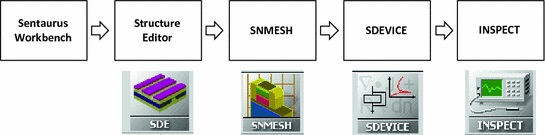
\includegraphics[width=15cm]{figure/TCAD.jpg}
  \caption{TCAD modules via Workbench}
\end{figure}

 \begin{figure}[hbt]
\centering
  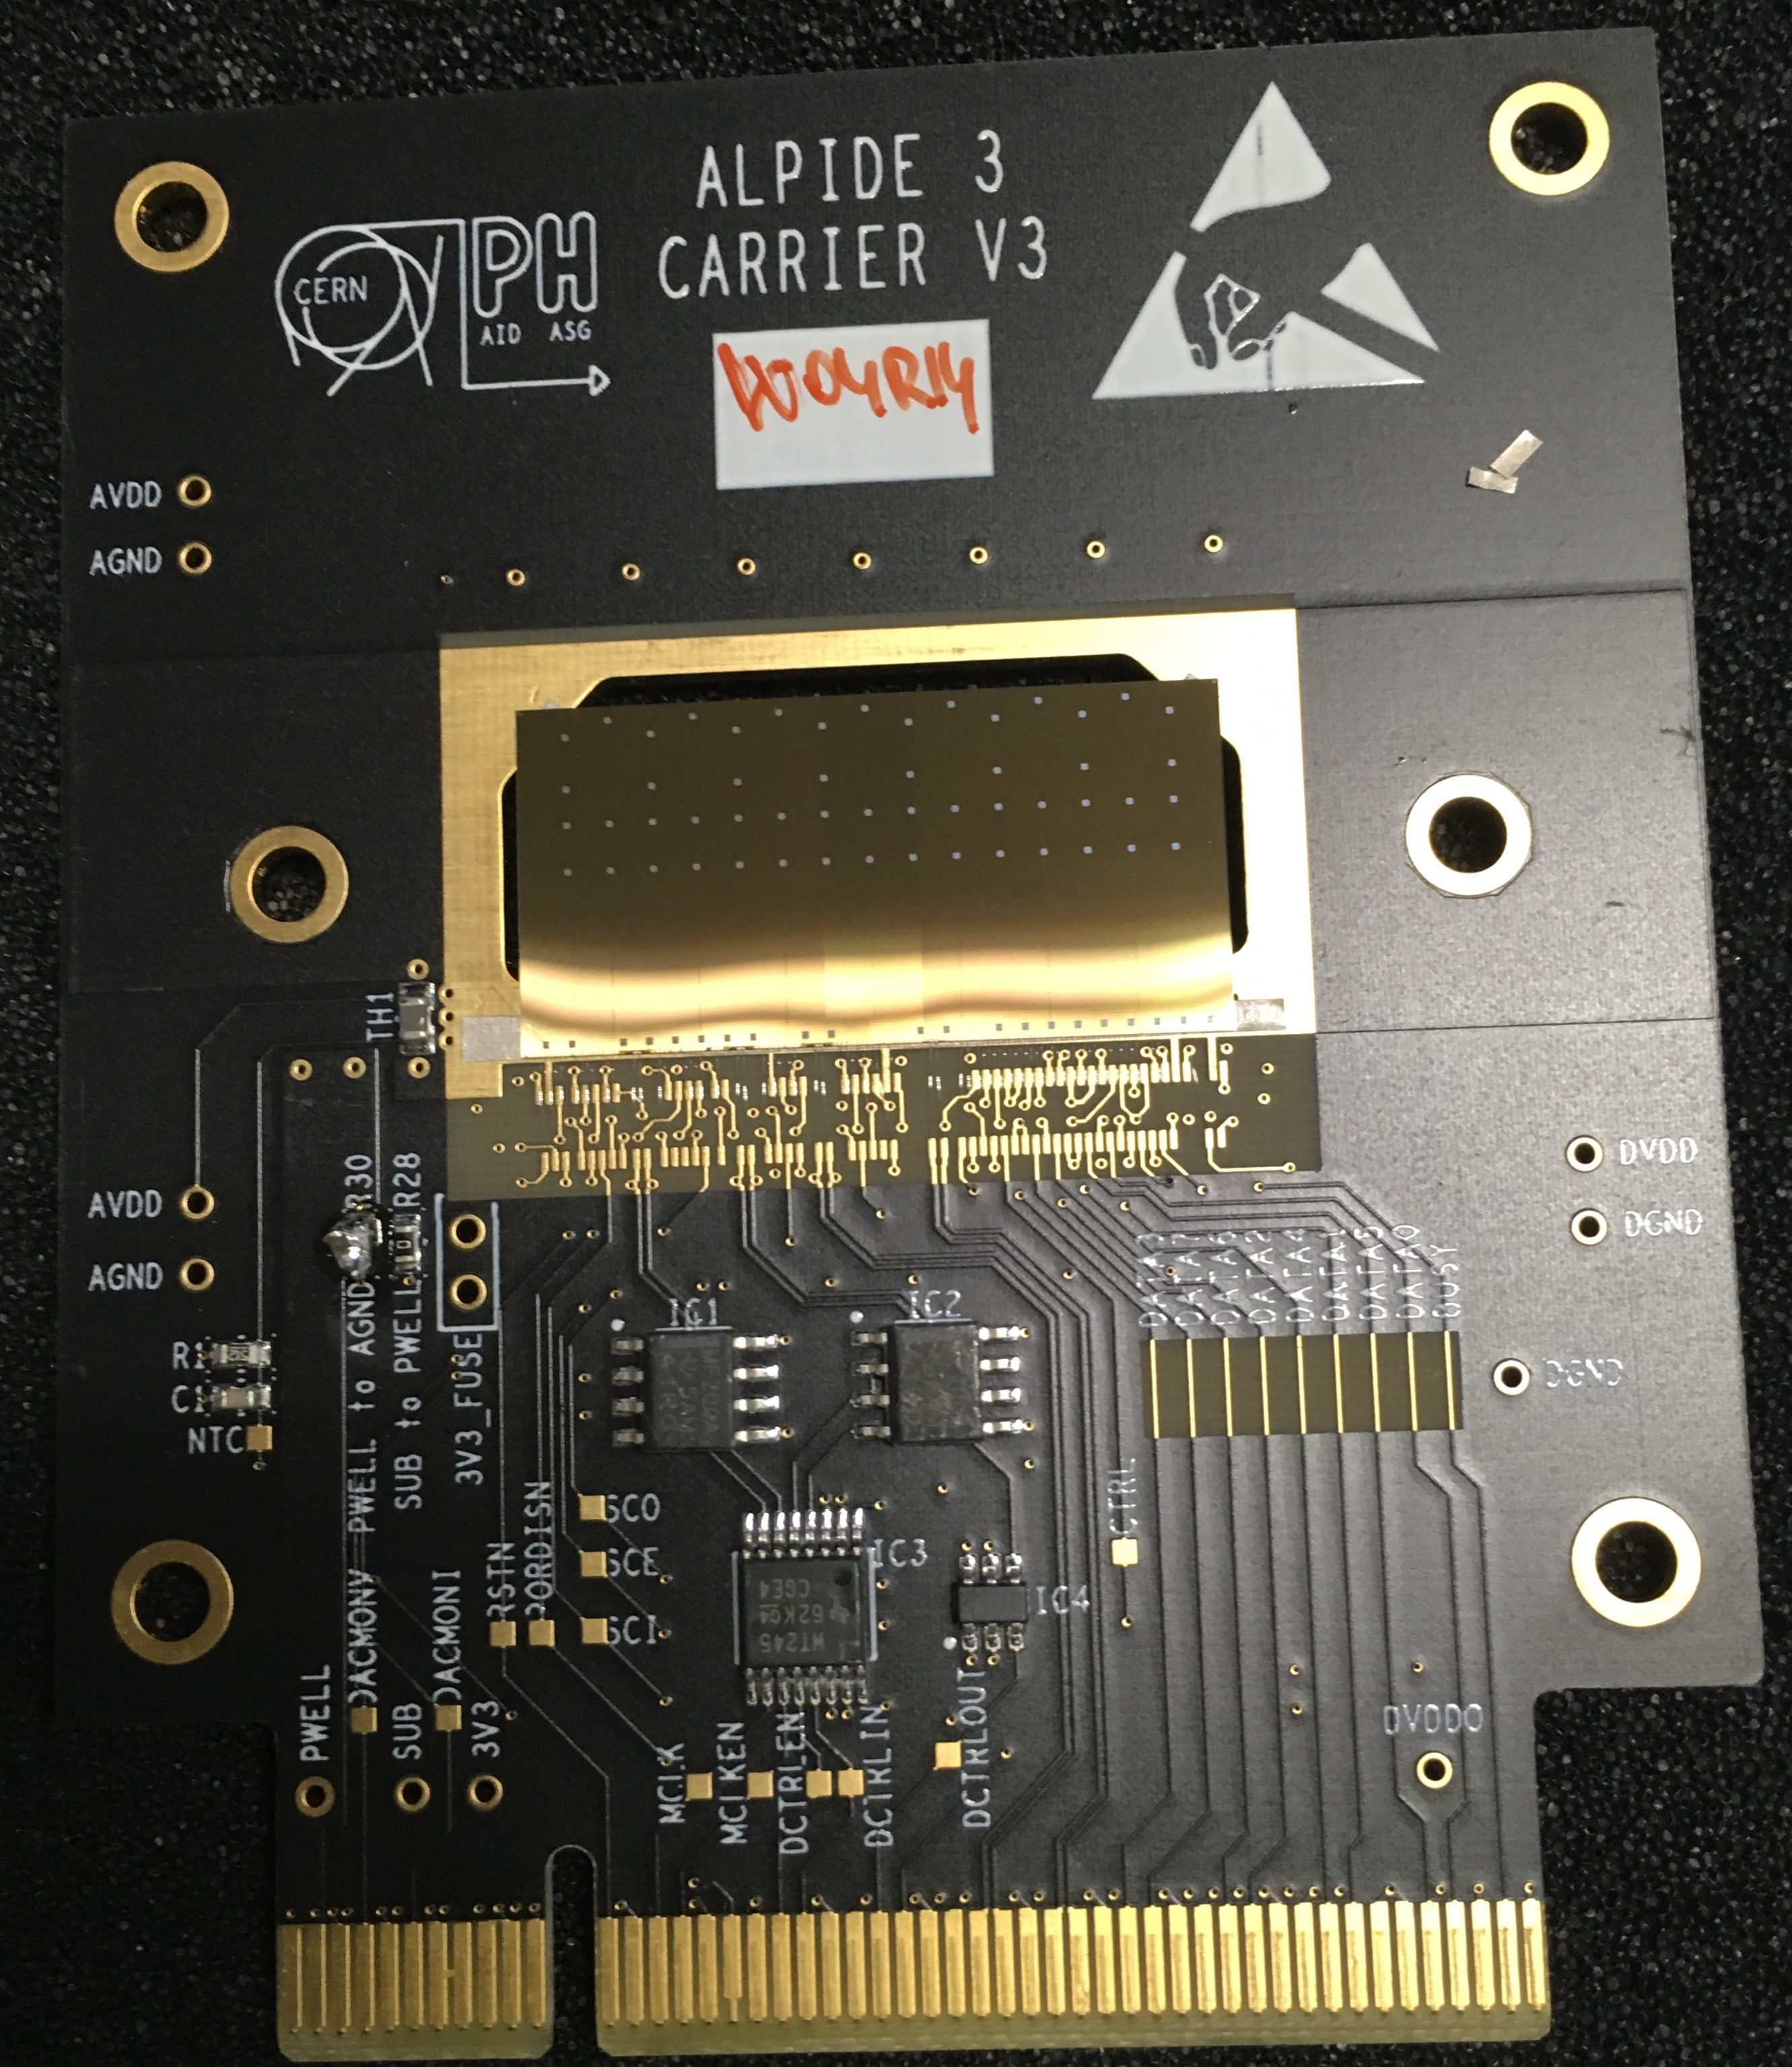
\includegraphics[width=7cm]{figure/ALPIDE3.jpg}
  \caption{ALPIDE single ship}
\end{figure}

\subsection{Introduction to Silicon}

\indent   Silicon is the dominant semiconductor material used in the production of position sensitive detectors for particle physics. The detection of minimum ionizing particles (MIP) is based on ionization or excitation of atoms in the medium caused by the passage of charged particles. Silicon which is a semiconductor material has 1.11 eV of energy gap at room temperature.  For its indirect band gap, the required energy for the transfer, not only given by the size of the band gap but additional energy has to be supplied to lift a valence electron into the conduction band, is 3.6 eV.

 \begin{figure}[hbt]
\centering
  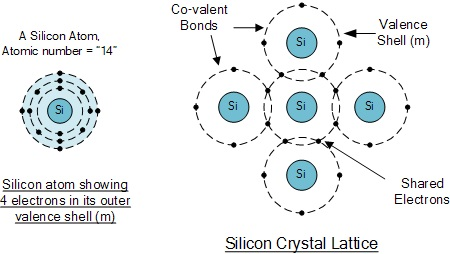
\includegraphics[width=12cm]{figure/diode1.jpg}
  \caption{Silicon structure\cite{Dragicevic:2010xca}.}
\end{figure}

\subsection{Radiation with Matter}

When a charged particle travels through  a medium, it loses energy due to interaction with  electrons and nuclei of atoms.     The interaction mechanisms depend upon the energy, the mass, the charge of the particle, and the characteristics of the medium. The interaction mechanisms are:

\begin{enumerate}
    \item Inelastic collisions with the atomic electrons of the material
    \item Elastic scattering from nuclei
    \item Nuclear reactions
    \item Emission of Cerenkov radiation
    \item Bremsstrahlung
\end{enumerate}

The interaction mechanisms of photons in the matter is entirely different from charged particles. Since the
photon does not have any electric charge, the inelastic collisions with electrons completely cannot occur. 
Although there is no inelastic collision, there still are important interaction mechanisms such as:

\begin{enumerate}
    \item Photoelectric effect
    \item Compton and Rayleigh scattering
    \item Pair production
\end{enumerate}

\subsubsection{Particle Radiation in Matter}

Radiation is detected by its interaction in the matter.  Interaction generates the signal which is read-out
and usually recorded. These interaction processes depend on both the type and the energy of the incoming
particles. The energy loss of incident particles, when they pass through the material,  can be determined by Bethe-Bloch equation (\ref{eq:Bethe-Bloch}). The equation \ref{eq:Bethe-Bloch} define the stopping power or the mean energy loss per unit length of incident massive charged particle.

\begin{equation}
    \label{eq:Bethe-Bloch}
    -\frac{dE}{dx} = 2\pi N_a r_e m_e c^2 \rho \frac{Z}{A} \frac{z^2}{\beta^2} \left[\ln{\frac{2m_e\gamma \nu W_{max}}{I^2}} - 2\beta^2 - \delta - 2\frac{C}{Z}\right]
\end{equation}

\begin{center}
\begin{table}[ht]
\resizebox{\textwidth}{!}{%
\begin{tabular}{ll}
    with:&\\
     $2\pi N_a r_e m_e c^2 = 0.1535$ MeVcm$^2$/g &  $\beta: c/v$ of incident particle\\
     $r_e$: electron radius ($2.817\times 10^{-13}$ cm)& $\rho$: density of absorbing material \\
     $m_e$: electron mass & $\gamma$: $1/\sqrt{1 - \beta^2}$\\
     $N_a$: Avogadro's number & $\delta$: density correction\\
     $Z$: atomic number of absorbing material & $C$: shell correction\\
     $A$: atomic weight of absorbing material & $I$: mean excitation potential\\
     $z$: charge of incident particle & $W_{max}$: maximum energy transferable \\
    & in single collision
\end{tabular}}
\end{table}    
\end{center}
where:
\begin{equation}
    \label{eq:Wmax}
    W_{max} = \frac{2m_ec^2\eta^2}{1 + 2s\sqrt{1 + \eta^2} + s^2}
\end{equation}
\noindent with $s = m_e/M$, $\eta = \beta \gamma$, and $M$ is particle mass.

The $I$ value indicates the mean energy for generating electron-hole pair in a semiconductor.  But there is no direct way to calculate the mean excitation potential.  However, the $I$ value of many materials can be observed from measurements.

\subsubsection{Multiple coulomb scattering}
When charged particles passing through materials, the interaction with nuclei produces the Coulomb scattering.  Since the nuclei  mass is greater than the incoming particle, the energy loss in the material is negligible but each scattering increases a small angle to the particle trajectory. Even if this change of the path of an incoming particle is small the sum of all the scattering make the particle trajectory  deviated from the initial incoming direction. 

\subsection{Carrier generation and transportation}
The free electron and hole can be generated by excitation energy from a number of mechanisms like thermal excitation or ionization by radiation. When free electron-hole pairs are produced their transportation within the medium contributes the signal in the semiconductor sensor. 

\subsubsection{Thermal generation}

In the semiconductor sensor, the thermal generation of free electron-hole contributes to  the noise in the detection signal .The thermal energy can excite the electron  to move from the valence band to the conduction band. For  the small band gap  material only the  thermal energy of T $= 300$K, it is enough to produce the noise signal at room temperature. In the case of the silicon sensor, although it  needs higher  energy to excite electron from the conduction band to the valence band due to its indirect band gap. However, the free   charged generation is also possible at  lower energy because of impurities and imperfect in the silicon lattice.
\subsubsection{Radiation generation}

The radiation generation is caused by the incoming photons and particles that interact with matter.  These process also generates the signal in the sensor. The mean energy ($W$) of excitation has to be higher than the energy band gap ($E_g$) as shown in equation \ref{eq:mean-en}, because it needs to excite phonon and plasmon states. Phonon excitation changes the energy of the lattice, then the energy appears as heat in the detector. The plasmon refers to the quantum state of the valence electron density oscillations with a mean energy of 17eV for silicon. Eventually, the mean energy that can be used for electron-hole creation is $W \approx 3.68$eV\cite{SiliconDetectorbook}.

\begin{equation}
    \label{eq:mean-en}
    W(E_g) = \left[1.76 + 1.84\cdot E_g\right]\mathrm{eV}
\end{equation}

\subsubsection{Drift transportation}

Free electrons in the material can move with the applied electric field. The mobile electrons can feel the force from the electric field, then they move to the opposite direction of the field. The movement direction depends upon the charge of the carrier, so the hole will move in the field direction, unlike electrons. The average of drift velocity for electron ($v_n$) and hole ($v_p$) are given by:
\begin{equation}
    \label{eq:vn}
    v_n = -\frac{q\tau_c}{m_n}E = -\mu_n E
\end{equation}\begin{equation}
    \label{eq:vp}
    v_p = -\frac{q\tau_c}{m_p}E = -\mu_p E
\end{equation}

The current densities can be written as :
\begin{equation}
    \label{eq:vn}
    J_n = -qnv_n = qn\mu_n E
\end{equation}
\begin{equation}
    \label{eq:vn}
    J_p = qnv_p = qn\mu_p E
\end{equation}

with E as a applied filed, q = $1.602\times 10^{-19}$ C, and the mean free time of free charge scatter in semiconductor at room temperature  $\tau_C \approx 10^{-12}$ s.

Carrier mobilities $\mu_n$ and $\mu_p$ depend upon temperature and impurity concentration because of the scattering of carrier in materials. In very high field, the mobilities become saturation $\mu_{n,s}$ and $\mu_{p,s}$.  

\subsubsection{Diffusion transportation}

The charge carrier can move from the higher concentration to lower concentration region, so the diffusion current is generated by the moving of charge carrier. The gradient of the concentration can be observed for diffusion current. If there is a high gradient concentration in the semiconductor device, the diffusion current is high. The similar thing happens with low gradient concentration because of the low diffusion current. The flux of charge carrier ($F_n$: electron, $F_p$: hole) can be described by the equations :

\begin{equation}
    \label{eq:Fn}
    F_n = - D_n	\bigtriangledown n
\end{equation}

\begin{equation}
    \label{eq:Fp}
    F_n = - D_p	\bigtriangledown p
\end{equation}

where $D_n$ and $D_p$ are diffusion constant of electron and hole respectively.
% % % % % % % % % % % % % % % section 6 % % % % % % % % % % % % % % %
\section{Scope and limitations}
In this thesis we plan to setup the pCT prototype in collaboration with University of Bergen using the ALPIDE chip from ALICE in the PSD part. Then, we will test the pCT prototype  at the the proton beam at King Chulalongkorn Memorial Hospital to obtain the information and limitation of the current ALPIDE sensor. And the final goal is to design a new MAPS sensor specifically for a pCT system using Sentaurus TCAD at TMEC. The details of scope and limitations are detailed below. 
 \begin{itemize}
      \item Working in collaboration with a research group at the University of Bergen to build the ALPIDE array chips to test with the  pCT prototype
      \item Connecting the ALPIDE sensors with the  Xilinx Virtex UltraScale+ FPGA VCU118 Evaluation Kit to test the communicate with  sensor arrays.
      \item The useful parameters for TCAD simulation will be extracted from the pCT prototype experiment.
      \item Working in collaboration with the Thai Microelectronics Center (TMEC) for sensor simulation and design. The three-dimensional model of the new sensor done by Sentaurus TCAD.
      \item Studying  the working condition of the pCT prototype with the proton beam at King Chulalongkorn Memorial Hospital 
      \item Comparing experimental results with simulation results from TCAD, Topas and Geant4
 \end{itemize}


% % % % % % % % % % % % % % % section 5 % % % % % % % % % % % % % % %

\section{Research procedure}
\subsection{Proton beam and facility}

\indent In the year 2020, there will be a Proton Therapy center in Thailand at King Chulalongkorn Memorial Hospital. It will be constructed in the celebration of 65 years anniversary of Her Royal Highness Princess Maha Chakri Sirindhorn. The beam is Cyclotron proton beam with the energy in the range of $70-245 $MeV which can be referred to 4-37 cm of water equivalence path length (WEPL). The diameter of the beam at isocenter is fewer than 5 mm by maximum energy and less than 7 mm by 100 MeV. The Proton flux density is $10^9$ proton/second at least. It  is a Hospital based Proton Therapy center with Single Gantry Scanning nozzle (IMPT) provided by Varian Proton Therapy Machine Model: Probeam Compact. The tracking system use real-time scanning with x-ray cone beam computed tomography (CBCT) imaging. The proton beam from this machine is the pencil scanning for mere treatment.    

\subsection{The ALPIDE sensor}

\indent ALPIDE is the  CMOS APS silicon sensor chip in the ITS2 detector.  Before the advent of the  ALPIDE chip, the ITS research teams of ALICE have been studied  the ULTIMATE sensor chip which is the first MAPS chip used in the Solenoidal Tracker (STAR), at the Relativistic Heavy Ion Collider (RHIC), Brookhaven National Laboratory, United States  
The first prototype of ALPIDE chip is called Explorer-0 which uses analogue readout with several geometries of pixel layouts.
It  is biased with revers bias on substrate of sensor chip. Explorer-1 is the next generation, the ALICE design team had tried  the new prototype with new pixel geometries, difference thickness and resistivity from Explorer-0. 
The 3rd prototype generation is pALPIDEss-0, it is the first prototype which combines buffering and discriminator into a chip and sparsified readout with zero suppression within the matrix. In 2013, ALICE achieved full pixels on single chip  called pALPIDE-1. As the 4th prototype, pALPIDE-1 composes of 512 rows x 1024 columns (double columns) of pixels and has bonding pad over the matrix. Next year after ALPIDE-1 was revealed, ALICE had pALPIDE-2 which was the 5th generation prototype and had final interface for ITS module constructing.
However,  it had slow speed of read out time. The Investigator was the 6th prototype and it was only constructed for study of pixel geometries and charge collection time. Finally, ALICE has succeed in the new prototype of sensor chip as 7th generation. The pALPIDE-3, it integrates 1.2 Gbit/s link and multiple event memories \cite{vanHoorn:2119197}, Final optimization of pixel and front-end and is prepared to ALPIDE which is real sensor chip in ITS nowadays.

\subsection{Experiments}

The University of Bergen is in the ALICE collaboration and  plan to use ALPIDE particle sensor in exploring the proton computed tomography properties. As  for SUT-ALICE collaboration, we are really interested in the application of pCT, and have been visited to the University of Bergen. It is interesting to find limitations of the current pCT prototype using the ALPIDE chip. To study ALPIDE chip in pCT environment, it could help the researcher in improving the design of the new dedicated MAPS  for pCT.

Xilinx VCU118 FPGA and ALICE ITS DAQ board can handle the communication of  multiple ALPIDE chips. Understanding of VCU118 can lead to the experiment for characterizing ALPIDE cable chip in pCT. The testing of ALPIDE chip with this board is constructed at University of Bergen and they have a plan to change from the sensor cable to be the array arrangement to increase the detection coverage area. Currently, the pCT  field programmable gate array (FPGA) firmware is still in development based on ALICE ITS firmware. SUT intends to help University of Bergen to install the array of ALPIDE  and  connect with VCU118.  The connection will be done using the transition card called FPGA Mezzanine Card (FMC) and firefly cables (ECUE-12-030-C1-FF-01-1, 
ECUE-12-100-C1-FF-01-1 and ECUE-12-200-C1-FF-01-1). 

For the RERD part, we will follow University of Bergen prototype to use the aluminium absorber as energy degrader instead a conventional crystal or   scintillator materials. This has some advantages since it can also serve as a mechanical carrier and cooling medium for the pixel sensors.

We will then set up an identical system to the one at University of Bergen and characterize the pCT prototype in two different tests, particle beam test and laboratory test.  Some parameters such as  cluster size, charge collection time, the number of tracked proton and some limitation of ALPIDE in the PSD setup will be obtained. The experiment will provide the limitations of ALPIDE for pCT and lead to the better specification of the new sensor which will be designed later using the TCAD software.  

\begin{figure}[hbt]
\centering
  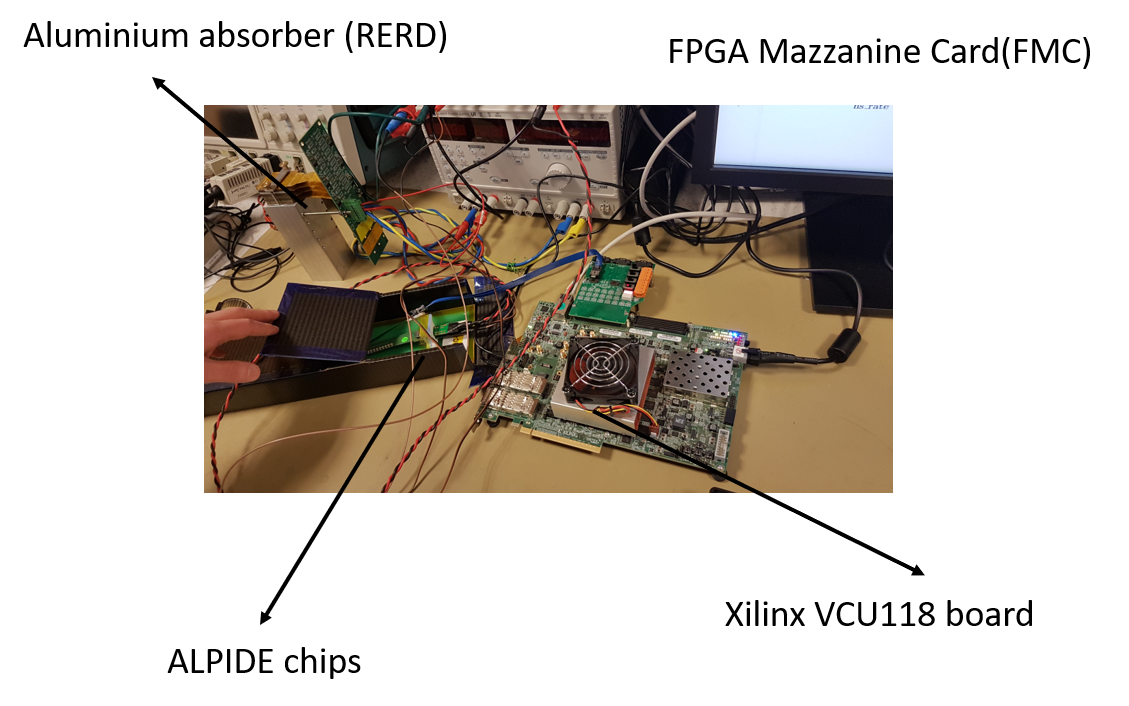
\includegraphics[width=10cm]{figure/PCTBergen.png}
  \caption{The pCT experiment at UiB}
  \label{fig:pCT}
\end{figure}

\subsection{Simulations}

There are several software packages that can be used to simulate the proton detector and proton computed tomography such as  FLUktuierende KAskade (Fluka), GEometry ANd Tracking (Geant ) and TOol for Particle Simulation (TOPAS).  Fluka is a particle physics Monte Carlo simulation package with applications in many areas including  high energy experimental physics, medical physics and radio-biology.   In the University of Bergen, there is a research group responsible for simulating particle detector and medical physics by using Geant4 and TOPAS. Geant4 mainly is a general purpose package designed for high energy physics while Topas extends the Geant4 Simulation Toolkit to focus on proton therapy. TOPAS results can provide the Digital Imaging and Communications in Medicine (DISCOM) which is the international standard to transmit, store, retrieve, print, process, and display medical imaging information.  

The TOPAS is useful if the ALPIDE and Xilinx VCU118 board are already fined for the pCT experiment. In the beginning phase of proton tracking at King Chulalongkorn Memorial Hospital, we still use the Geant4 simulation as a main simulation software. Another advantage of Geant4  over TOPAS is that its result can be compared to the TCAD simulation of charge collection. Moreover, the counting of proton in a frame is also possible to calculate by Geant4. 

TCAD is a computer simulation software that helps to model, develop and optimize semiconductor processing and semiconductor device design. There are a number of Proprietary TCAD software providing the complete solution to the industry.   By collaboration with TMEC, we are able to use the Sentaurus TCAD Software for our semiconductor and device simulation.  The use of TCAD software will be able to perform the simulation of charge collection, carrier spreading, I-V characteristics, cluster size, and proton radiation damage of a new design sensor of a pCT prototype. The simulated results will be compared with the experiment results. In case of the  ALPIDE the simulation results from Sentaurus TCAD software are in good agreement with characterization results obtained from both beam test and laboratory test. 

% % % % % % % % % % % % % % % section 7 % % % % % % % % % % % % % % %
\newpage
\begin{landscape}
\section{Research Schedule}
 \begin{table}[!h]
 \small
% \caption{Research Schedule}
\begin{tabular}{|l|l|l|l|l|l|l|l|l|l|l|l|l|l|l|l|}
\hline
\multirow{2}{*}{\diagbox[height=1.2\rotheadsize, width=\dimexpr\eqboxwidth{AB}+50\tabcolsep\relax]%
    {\raisebox{1.5ex}{Topic}}{\raisebox{-1ex}{Semester}}} & \multicolumn{3}{c|}{2016} & \multicolumn{3}{c|}{2017} & \multicolumn{3}{c|}{2018} & \multicolumn{3}{c|}{2019} & \multicolumn{3}{c|}{2020} \\ \cline{2-16} 
 
&1       &    2   &    3   &     1  &    2   &    3   &    1   &    2   &    3   &   1    &  2     &  3     &    1   &    2   &   3    \\ \hline
 
1) Literature Review&  \checkmark     &  \checkmark     & \checkmark      &       &  \checkmark     & \checkmark      & \checkmark       & \checkmark       &       &      &      &      &       &       &       \\ \hline
 
2) Studying in 1D TCAD simulation at TMEC&       &       &       &  \checkmark     &       &       &       &       &       &       &       &       &       &       &       \\ \hline

3) Studying ALPIDE characterization laboratory&       &       &       &       &       &       &       &       &       &       &       &      &      &       &       \\ 
\hspace{0.4cm}in University of BergenD&       &       &       &       &       &       &     &      &        & \checkmark      & \checkmark      &      &       &       &       \\\hline

4) Constructing ALPIDE characterization in &       &       &       &       &       &       &       &       &       &      &       &       &       &       &       \\ 
\hspace{0.4cm}array laboratory at Suranaree University of &       &       &       &       &       &       &       &       &       &      &      &  \checkmark     &  \checkmark       &       &       \\
\hspace{0.4cm}Technology&       &       &       &       &       &       &       &       &       &       &       &       &       &       &       \\\hline
 
5)Modelling and simulation of proton sensor in pCT&       &       &       &       &       &       &       &       &       &       &       &      &  \checkmark     & \checkmark     & \\\hline
 
6) Thesis writing&       &       &       &       &       &       &       &       &       &       &   \checkmark    &  \checkmark     &  \checkmark     &   \checkmark    &   \checkmark  \\ \hline
\end{tabular}
\end{table}
\end{landscape}
\newpage

%%%%%%%%%%%%%%%%%%%%%%%%%%%%%%%%%%%%%section 8%%%%%%%%%%%%%%%%%%%%%%%%%%%%%%%%%%%%%%%


\section{Expected results}
\begin{enumerate}
\item The front-end sensor specification for the pCT prototype.
\item The firmware of programmable DAQ(Xilinx VCU118) for the pCT prototype
\item Limitations of the ALPIDE chip in the pCT prototype. 
\item Important parameters that can be used as input to optimize  the new MAPS design of the pCT system.
\item The TCAD models and simulation results for the better PSD sensor of the pCT system.
\end{enumerate}

%%%%%%%%%%%%%%%%%%%%%%%%%%%%%%%%%%%%%%section 10%%%%%%%%%%%%%%%%%%%%%%%%%
\section{Acknowledgements}

I would like to thank  Mr.Wittawat Yamwong from TMEC for TCAD training and Professor Dr. Dieter Rorich from University of Bergen who gives me an opportunity to work in his laboratory. Finally, I really appreciate the Development and Promotion of Science and Technology Talents Project scholarship (DPST) and Thailand Center of Excellence in Physics (ThEP-61-PHM-SUT4) for financial support.

\newpage
\bibliographystyle{aplike}
\bibliography{pokref.bib}
\end{document} 

